% !TeX encoding = UTF-8
%


% Besserer Vorschlag: 
% Screenshot von ReportGenerator
% sieht schöner aus ...
% zum Schluss machen und einfach als Bild
% einfügen!

% TODO: Seitennummern!



\subsection{Abdeckung}
\label{Abschnitt:Tests:Statistik:Abdeckung}


Auf den folgenden Seiten steht der aus den Daten von OpenCover generierte Bericht zur Testabdeckung durch Komponententests.


%\newgeometry{left=8cm,bottom=0.1cm,top=1cm,right=0.1cm}
\newgeometry{includehead,includefoot,
  left=1.in,right=1.0in,
  top=0.6in,bottom=0.8in,
  headheight=20pt,headsep=0.25in,
  footskip=0.3in}

\thispagestyle{empty}
\pagestyle{empty}

\begin{figure}[h!]

	\centering{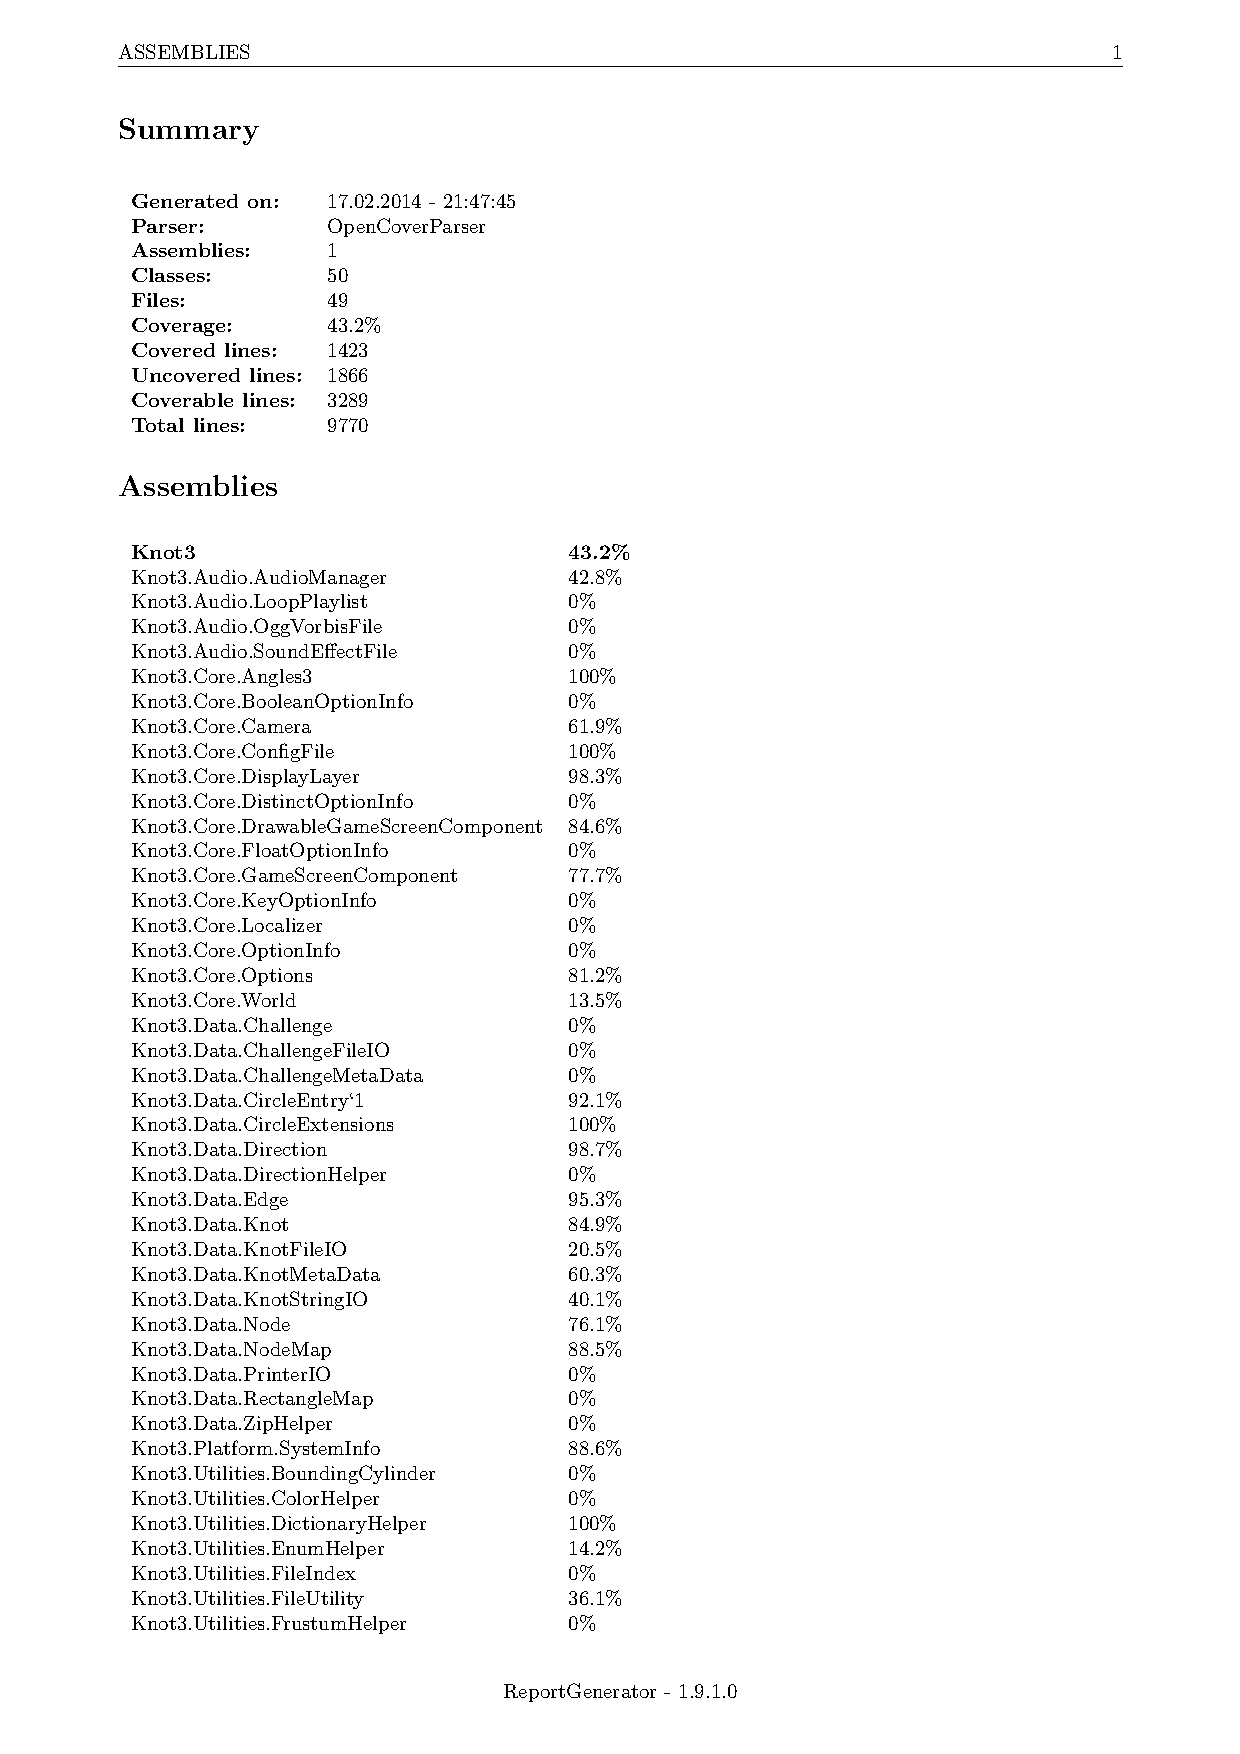
\includegraphics[page=1,scale=1.0]{Inhalt/Tests/Abdeckung/OpenCover_Bericht_uebersicht.pdf}} 
   
\end{figure}


%\begin{figure}[h!]
%
%	\centering{\includegraphics[page=2,scale=1.0]{Inhalt/Tests/Abdeckung/OpenCover_Bericht_uebersicht.pdf}} 
%   
%\end{figure}

\restoregeometry